
\documentclass{article} % For LaTeX2e
\usepackage{style,times}
\usepackage{amsmath,amsfonts,bm,amssymb}


%%%%% customized by shuo begin
\usepackage{amsthm, hyperref, url, csquotes, dsfont}
\usepackage{tikz}
\DeclareMathOperator*{\argmax}{argmax}
\DeclareMathOperator*{\softmax}{softmax}

\newtheorem{theorem}{Theorem}
\newtheorem{definition}{Definition}
\newtheorem{proposition}{Proposition}
\newtheorem{example}{Example}

\newcommand{\red}[1]{\textcolor{red}{#1}}
\newcommand{\blue}[1]{\textcolor{blue}{#1}}
%%%% customized by shuo end

\title{Reward Modeling in LLM Alignment}
\author{Shuo Liu \\
Computer Science\\
Northeastern University\\
\texttt{shuo.liu2@northeastern.edu} \\
}

\iclrfinalcopy % Uncomment for camera-ready version, but NOT for submission.
\begin{document}

\maketitle

\begin{abstract}
	Constructing rewards is crucial yet challenging to achieve RL objectives. This post explores how to guide the LLM optimization via a proper RLHF reward model.
\end{abstract}

\section{Reward Models in RLHF}

As LLMs scale, their raw outputs (optimized primarily for next-token prediction) often diverge from expected traits. To enable RL fine-tuning from human feedbacks (RLHF), reward models are introduced as trainable proxies for human preference. Once trained, it can generalize preference signals to unseen inputs, making alignment more scalable by reducing reliance on slow and costly human annotations. It also allows flexible fine-tuning toward different objectives, such as helpfulness, truthfulness, or safety.

A typical alignment pipeline consists of 3 stages: supervised fine-tuning (SFT), reward modeling, and RL. After an initial SFT based on base transformer with curated human-labeled data, a reward model is constructed to predict human preferences over model-generated responses. This model is then used to guide further optimization by encouraging outputs that maximize the predicted reward. For example, \texttt{ChatGPT} employs reward models trained on ranked annotations to guide its generation toward preferred outputs \cite{openai2024gpt4technicalreport}; \texttt{DeepSeek} and \texttt{LLaMA 2} include explicit reward modeling components in their alignment pipelines, using pairwise preferences to train reward models that inform subsequent learning \cite{shao2024deepseekmathpushinglimitsmathematical, llama}.

\begin{figure}[hbt]
\centering
  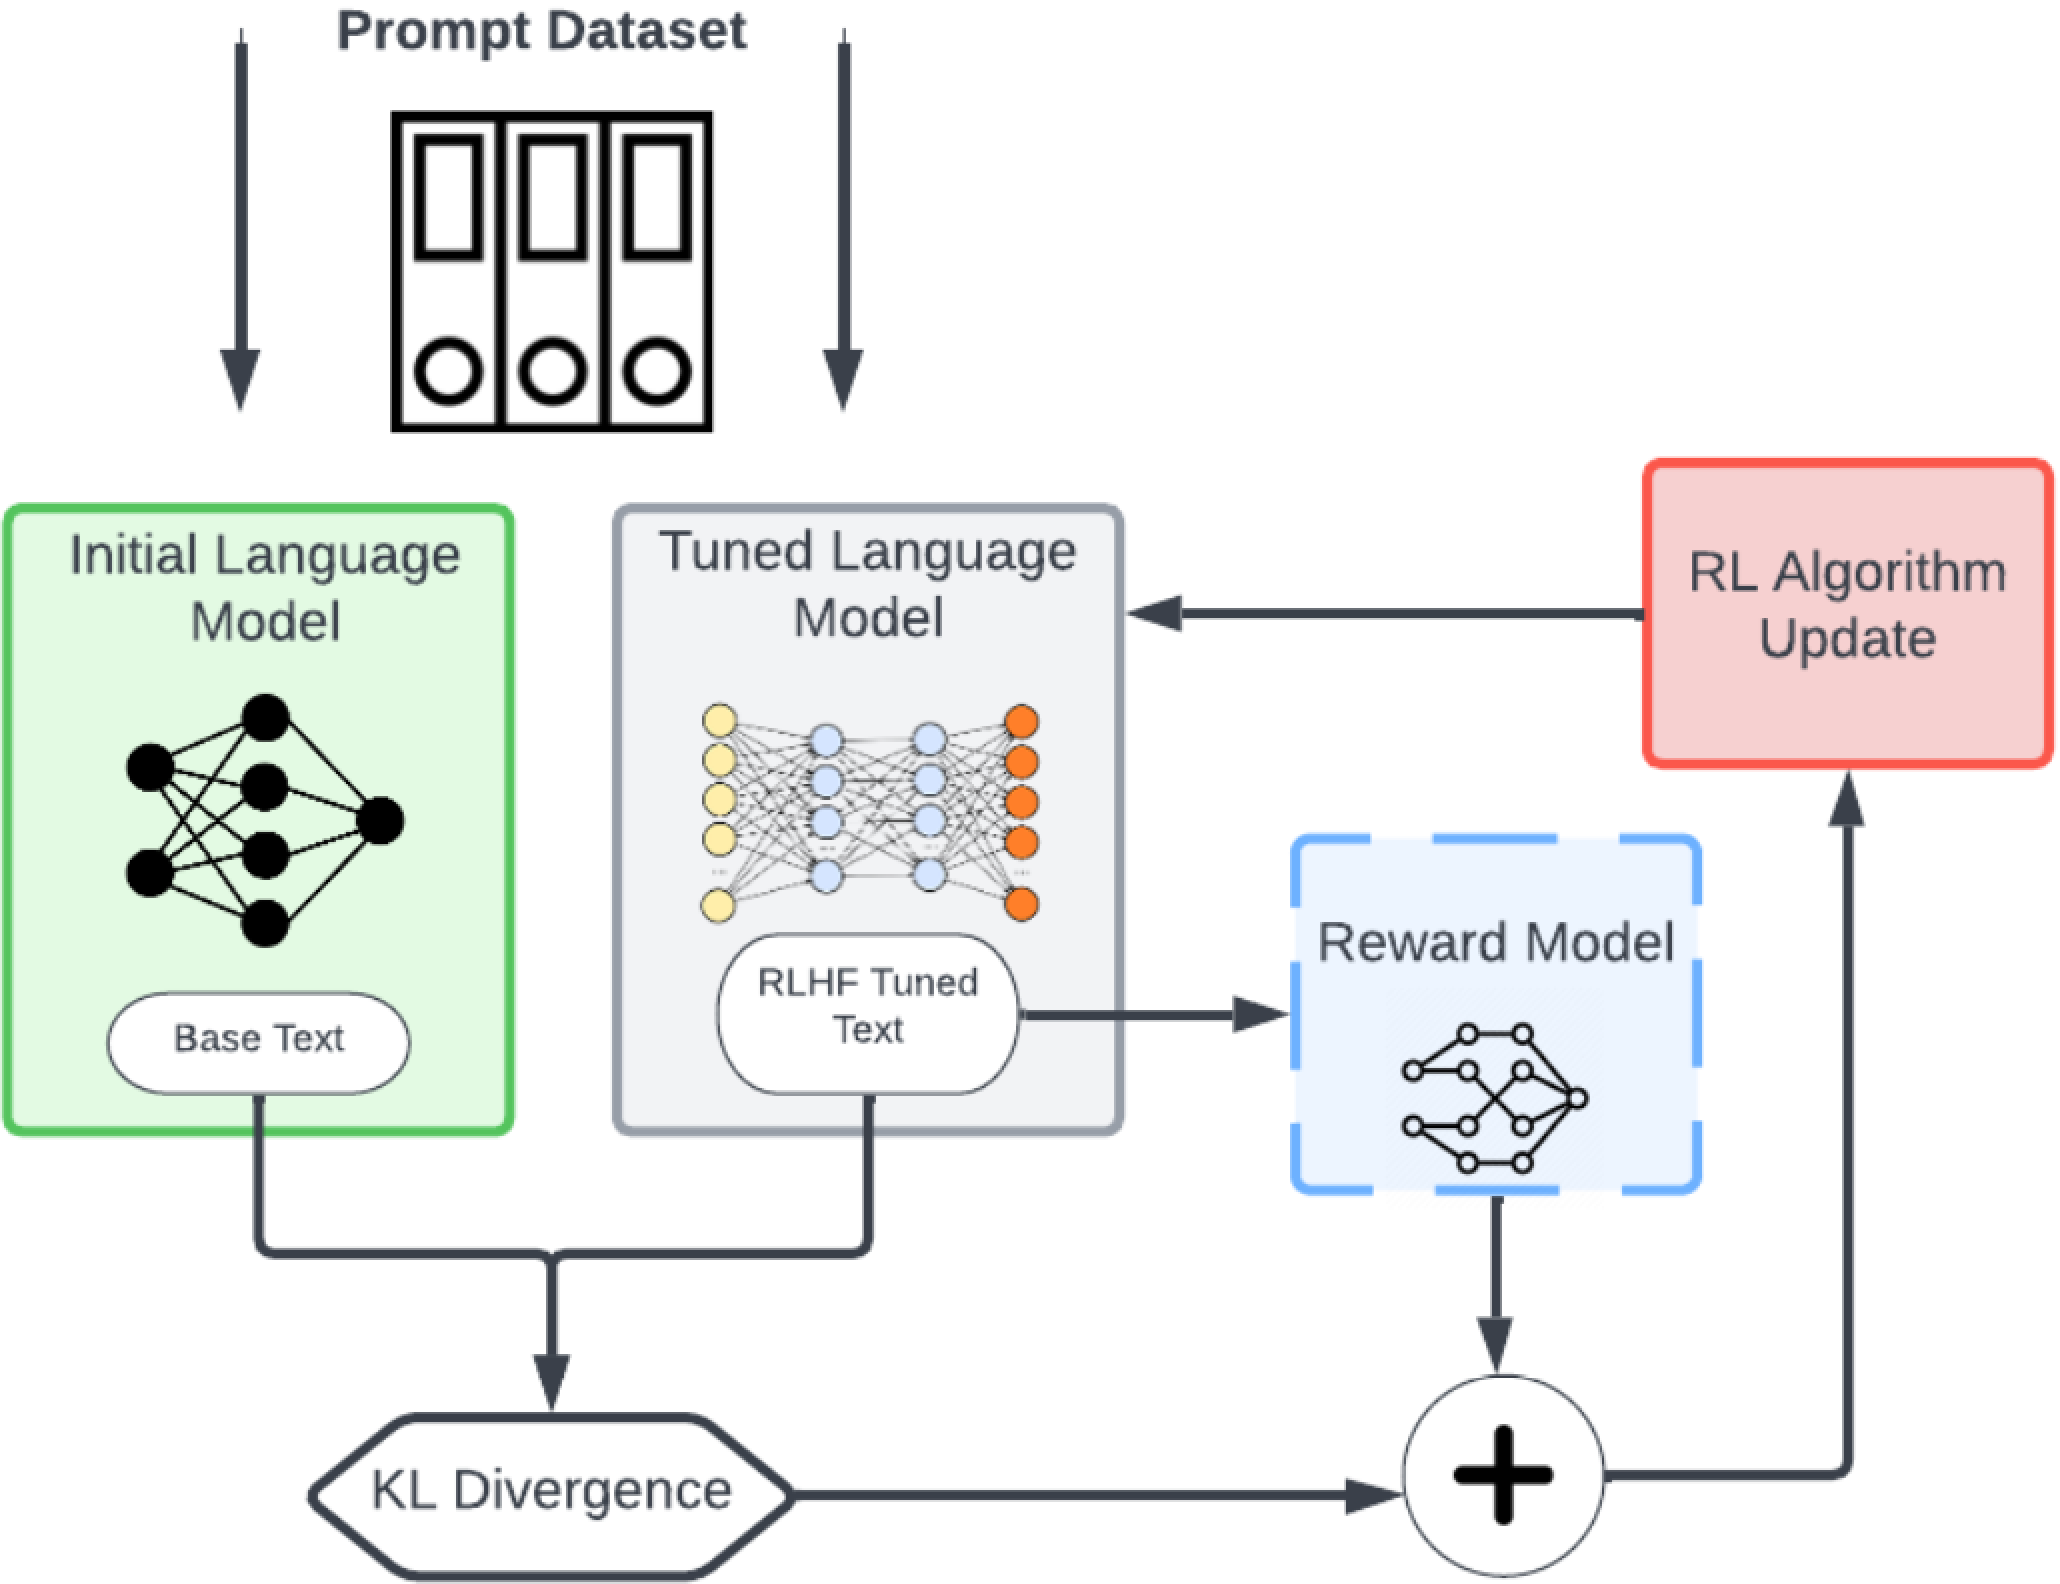
\includegraphics[width=0.6\linewidth,height=0.44\linewidth]{RLHF.png}
  \caption{Role of the reward models in RLHF (reward model \blue{in blue}).}
\end{figure}

\section{Anti-Symmetric Preference Modeling}

In this section, we introduce the mainstream methods that model rewards of LLM responses through preference comparison.

\subsection{BT Model and Its Ranking Extension}

The original Bradley-Terry (BT) model posits that, given a pair of options $i$ and $j$ drawn from some population, the probability of selecting $i$ is,
\begin{equation}
	\Pr(i \succ j) = \frac{u_i}{u_i + u_j}=\frac{\exp(r(i))}{\exp(r(i)) + \exp(r(j))}, \label{eq:bt}
\end{equation}
where $u_i$ and $u_j$ are the respective utility or preference of options $i$ and $j$, which commonly parameterized in the exponential form via rewards $r(i)$ and $r(j)$. It can be further extended to rank $N$ options, known as Plackett-–Luce (PL) model,
\begin{equation}
	\Pr(i_1 \succ i_2 \succ \cdots \succ i_N) = \prod_{k=1}^{N} \frac{\exp(r(i_k))}{\sum_{j=k}^{N} \exp(r(i_j))}. \label{eq:pl}
\end{equation}
BT model is anti-symmetric, which means the preference between two responses depends only on the difference in their reward values. It satisfies $\Pr(y_i \succ y_j) = 1 - \Pr(y_j \succ y_i)$, and the log-odds of preference is anti-symmetric: $\log \left( \frac{\Pr(y_i \succ y_j)}{\Pr(y_j \succ y_i)} \right) = r(x, y_i) - r(x, y_j)$. This structure ensures consistent and transitive pairwise comparisons, making BT suitable for preference modeling. This is initially used to rank sports teams and players, i.e., Elo rating system.

\subsection{Reward Modeling with Pairwise Preferences (BT Model)}

Inferring a reward model using the BT framework can be formulated as a parameter estimation problem, where the objective is to recover latent reward values for candidate responses based on observed pairwise comparisons.

Suppose a prompt $x$ is associated with $N$ candidate responses $\{y_1, \cdots, y_N\}$, and human annotators provide preference labels between some pairs. Ideally, given sufficiently many comparisons under deterministic preference, the true reward values can be accurately inferred.\footnote{$O(N \log N)$ comparisons are sufficient for modeling rewards of $N$ responses.} In practice, however, this inference is challenged by stochastic human behavior and sparse annotation.

\paragraph{Modeling Assumptions} 
To make BT applicable to reward modeling under the practical conditions, we adopt the following assumptions \cite{sun2025rethinkingbradleyterrymodelspreferencebased}:
\begin{enumerate}
    \item \texttt{Deterministic responses and rewards:} For a given prompt $x$, a response $y$ is deterministically generated by a model. The oracle reward $r(x, y)$ associated with each prompt-response pair is fixed.
    \item \texttt{Deterministic annotators with bounded bias:} When a an annotator $A$ compares responses, their preferences are deterministically depending on the comparison of their biased evaluation of the reward,
    \begin{equation}
        \mathds{1} ( \underbrace{y_i \succ y_j}_\text{decision} | x, A ) = \mathds{1} (\underbrace{r(x,y_i) + b(x, y_i; A) > r(x,y_j) + b(x, y_j; A)}_\text{biased preference} ).
    \end{equation}
    
    \item \texttt{Order-preserving shaping:} To address sparsity in comparisons, a known embedding function $\Psi$ is assumed to map each $(x, y)$ pair into a feature space, with the constraint that $\Psi$ is order-preserving and does not affect optimization. High-dimensional embeddings can be beneficial because they increase the likelihood that semantically similar prompt-response pairs are mapped to nearby regions in the embedding space, thereby enabling comparisons to generalize more effectively. Though, it also introduces potential issues such as \textit{reward hacking} (Section~\ref{app:reward_hacking}).

    \item \texttt{Imperfect human annotations}: The annotator function $h(x_1, x_2, y_1, y_2)$ provides feedback that possibly aligns with the oracle reward $r(x, y)$. And it is harder to assign correctly when the reward difference between two pairs is small,
\begin{equation}
\mathbb{P}\left( h(x_1, x_2, y_1, y_2)(r(x_1, y_1) - r(x_2, y_2)) > 0 \,\middle|\, \Delta r \right) = \xi(\Delta r), 
\end{equation}
where $\Delta r := |r(x_1, y_1) - r(x_2, y_2)|$ is the reward difference, and $\xi$ is any monotonic increasing function to $[0.5, 1]$.
\end{enumerate}

\paragraph{Likelihood and Estimation}
Let each observed preference be denoted as a pair $(i \succ j)$, indicating that $y_i$ is preferred over $y_j$ for prompt $x$. Under the BT model, the probability of this outcome is,
\begin{equation}
    \Pr(y_i \succ y_j | x) = \frac{\exp(r(x, y_i))}{\exp(r(x, y_i)) + \exp(r(x, y_j))}.
\end{equation}
Given a dataset of $M$ annotated comparisons $\mathcal{C} = \{(i_m, j_m)\}_{m=1}^M$, the likelihood of observing these preferences is,
\begin{equation}
    \mathcal{L}(r) = \prod_{m=1}^M \frac{\exp(r(x, y_{i_m}))}{\exp(r(x, y_{i_m})) + \exp(r(x, y_{j_m}))},
\end{equation}
and the corresponding log-likelihood is,
\begin{equation}
    \log \mathcal{L}(r) = \sum_{m=1}^M \left[ r(x, y_{i_m}) - \log\left(\exp(r(x, y_{i_m})) + \exp(r(x, y_{j_m}))\right) \right].
\end{equation}
The optimal reward model is then obtained by maximizing the log-likelihood (MLE),
\begin{equation}
    r^* = \argmax_r \log \mathcal{L}(r).
\end{equation}
The solution is identifiable up to an additive constant and converges to the ground-truth rewards under the assumptions above.

\subsection{Reward Modeling with Ranked Preferences (PL Model)}

While the BT model provides a principled way to infer rewards from pairwise preferences, real-world systems can collect richer feedback in the form of ranked lists. Human annotators are presented with multiple responses to the same prompt and asked to provide an overall ranking. The reward model is then trained to assign scores that agree with these rankings.

PL model Equation.~\ref{eq:pl} is used in a similar way for MLE, just like BT model. For a ranking of alternatives $(y_{i_1} \succ y_{i_2} \succ \ldots \succ y_{i_N})$ for prompt $x$, the probability under the PL model is,
\begin{equation}
	\Pr(y_{i_1} \succ y_{i_2} \succ \ldots \succ y_{i_N} | x) = \prod_{k=1}^{N-1} \frac{\exp(r(x, y_{i_k}))}{\sum_{j=k}^{N} \exp(r(x, y_{i_j}))}.
\end{equation}
Given a dataset of $M$ rankings $\mathcal{C} = \{(y_{i_1^m}, y_{i_2^m}, \ldots, y_{i_{N_m}^m})\}_{m=1}^M$, the likelihood is,
\begin{equation}
	\mathcal{L}(r) = \prod_{m=1}^{M} \prod_{k=1}^{N_m-1} \frac{\exp(r(x, y_{i_k^m}))}{\sum_{j=k}^{N_m} \exp(r(x, y_{i_j^m}))}.
\end{equation}
And the corresponding log-likelihood is,
\begin{equation}
\log \mathcal{L}(r) = \sum_{m=1}^{M} \sum_{k=1}^{N_m-1} \left[ r(x, y_{i_k^m}) - \log\left(\sum_{j=k}^{N_m} \exp(r(x, y_{i_j^m}))\right) \right].
\end{equation}
The optimal reward model is then obtained by MLE,
\begin{equation}
r^* = \underset{r}{\arg\max} \log \mathcal{L}(r).
\end{equation}

Preference modeling with the PL model is also anti-symmetric, swapping the order of two responses in the ranking inverts the relative score difference in the likelihood expression.


\newpage
\section{Symmetric Reward Modeling}

As cliché as it sounds, modeling rewards of LLM responses through symmetric preference signals is indeed feasible. Symmetric models predict the reward for each prompt-response pair independently, without reference to alternative responses.

\subsection{Regression-based Reward Model}

A common symmetric approach is to train a regression-based reward model on scalar human ratings. Given a dataset $\{(x_n, y_n, s_n)\}_{n=1}^N$, where $s_n \in \mathbb{R}$ denotes the score assigned to response $y_n$ for prompt $x_n$, the reward model $r(x, y)$ is trained to minimize a squared loss:
\begin{equation}
    \mathcal{L}_{\text{reg}} = \sum_{n=1}^N \left(r(x_n, y_n) - s_n\right)^2.
\end{equation}
Such scalar-labeled data is available in open datasets like \texttt{Anthropic HH}, \texttt{OpenAssistant}, and \texttt{MT-Bench}, where annotators assign numeric quality scores to individual responses without ranking alternatives.

\subsection{Classification-based Reward Model}

Alternatively, a reward model can be trained as a binary classifier to predict whether a response satisfies certain alignment criteria (e.g., helpfulness or harmlessness). In this case, binary labels $s_n \in \{0, 1\}$ indicate whether a response is considered acceptable, and the reward model is trained using a standard cross-entropy loss with sigmoid $\sigma$ activation,
\begin{equation}
    \mathcal{L}_{\text{cls}} = - \sum_{n=1}^N \left[ s_n \log \sigma(r(x_n, y_n)) + (1 - s_n) \log(1 - \sigma(r(x_n, y_n))) \right].
\end{equation}


\section{Other Reward Modeling Techniques}

\subsection{Inverse Reinforcement Learning}

Inverse Reinforcement Learning (IRL) aims to recover an underlying reward function that explains the behavior of an expert operating within a MDP. Formally, consider an MDP defined by the tuple $(\mathcal{X}, \mathcal{Y}, T, \gamma)$, where $\mathcal{X}$ is the set of states, $\mathcal{Y}$ the set of actions, $T(x' | x, y)$ the transition dynamics, and $\gamma$ the discount factor. Given a set of expert trajectories ${\tau_i}$, where each trajectory $\tau_i = (x_0, y_0, x_1, y_1, \dots)$, the goal of IRL is to infer a reward function $r: \mathcal{X} \times \mathcal{Y} \rightarrow \mathbb{R}$ such that the optimal policy induced by this reward function explains the observed expert behavior. However, this does not match seamlessly for reward modeling in LLM alignment due to,
\begin{itemize}
    \item \texttt{Unstructuredness:} IRL assumes access to expert trajectories in a well-defined MDP, which does not align with the unstructured, high-dimensional nature of language modeling.
    \item \texttt{Incompatible feedback format:} Human feedback for LLMs is typically given as relative preferences between completions rather than as optimal action sequences.
    \item \texttt{Huge computation:} IRL methods are computationally expensive and require solving RL problems repeatedly, which is impractical for large-scale language models.
\end{itemize}

\subsection{Bayesian Reward Learning}

Bayesian reward learning explicitly represents uncertainty about the reward function by maintaining a posterior distribution $p(\theta | D)$ over reward parameters $\theta$, given observed demonstration data $D$. Using Bayesian inference, it updates a prior distribution $p(\theta)$ to a posterior, $p(\theta | D) \propto p(D | \theta) p(\theta)$
allowing the derived policy to incorporate uncertainty (e.g., via posterior sampling). However, Bayesian inference in high-dimensional reward spaces is computationally expensive and impractical for large-scale LLMs, since the exact posterior inference is often intractable.

\newpage
\section{Takeaways in Reward Design} \label{app:reward_hacking}

Effective reward design is critical in guiding RL agents towards desirable behaviors. Several considerations and specialized techniques help ensure robust and aligned outcomes. Here are some specific takeaways should be considered when designing rewards.

\paragraph{Potential-based Reward Shaping}
Reward shaping accelerates learning by augmenting the original reward with additional informative signals. Potential-based shaping ensures optimal policy invariance by defining additional rewards through a state-dependent potential function $\Phi(s)$. Specifically, the shaping reward is formulated as $F(s, a, s') = \gamma \Phi(s') - \Phi(s)$, thereby avoiding the introduction of unintended behaviors or reward hacking vulnerabilities.
\begin{quote}
\scriptsize
	\enquote{\texttt{\textit{Rubric engineering is the new prompt engineering.}}} \hfill -- \texttt{\textit{Will Brown}}.
\end{quote}

\paragraph{Sparse vs. Dense Rewards}
The frequency and clarity of feedback significantly influence learning efficiency and agent behaviors. Sparse rewards, given infrequently and typically at task completion, mitigate reward hacking risks but pose exploration challenges \cite{weng2024rewardhack}.\footnote{The ambiguous or underspecified rewards design that creates vulnerabilities for agents' exploitation.} Conversely, dense rewards provide frequent feedback that facilitates exploration yet may inadvertently encourage reward exploitation or unintended optimization behaviors.

\paragraph{Human-in-the-loop Reward Design}
Incorporating human judgments directly into reward signals enables iterative refinement, capturing nuanced and complex objectives not easily formalized. Human-in-the-loop methods mitigate reward hacking by continuously aligning rewards with intended outcomes through active human oversight.

\paragraph{Intrinsic vs. Extrinsic Rewards}
Intrinsic rewards originate internally, driven by agent behaviors such as curiosity or novelty-seeking, promoting adaptive and exploratory capabilities. Extrinsic rewards come externally, explicitly set by designers. A balanced integration of intrinsic and extrinsic rewards supports robust agent behaviors through diversified motivational signals.


\bibliography{ref}
\bibliographystyle{ref}
%\newpage
\appendix
\section{Omitted Proofs}

This section shows the omitted (but non-trivial) proofs.

\subsection{Proof Theorem~\ref{them:PG}}
\begin{proof}
The gradient of $V$ function can be written in terms of $Q$ function,

{\footnotesize
    \begin{equation}
        \begin{aligned}
            \nabla V^{\pi}(s) &= \nabla\left [ \sum_a \pi(a|s) Q^\pi (s,a)\right ] \\
            &=\sum_a\left [ \nabla\pi(a|s) Q^\pi (s,a) +\pi(a|s) \nabla Q^\pi (s,a) \right] \\
            &=\sum_a\left [ \nabla\pi(a|s) Q^\pi (s,a) +\pi(a|s) \nabla \sum_{s'}P(s'|s, a)(r+V^\pi(s')) \right] \\
            &\stackrel{\text{(i)}}{=}\sum_a\left [ \nabla\pi(a|s) Q^\pi (s,a) +\pi(a|s) \sum_{s'}P(s'|s, a)\nabla V^\pi(s') \right ], \\
        \end{aligned}\nonumber
    \end{equation}
}
where we can have the derivation (i) since $r$ only depends on the environment dynamics.

Let $\phi(s) = \sum_a \nabla\pi(a|s) Q^\pi (s,a)$. We use $\rho^\pi(s\rightarrow x, k)$ to represent the probability of transitioning from state $s$ to $x$ with policy $\pi$ after $k$ steps, i.e., $\rho^\pi(s \rightarrow s', 1)=\sum_a \pi(a|s) P(s'|s, a)$. Thus, we can unroll the recursive form as below,

{\footnotesize
    \begin{equation} 
        \begin{aligned}
            \nabla V^{\pi}(s) &=\phi(s) +\sum_a \pi(a|s) \sum_{s'}P(s'|s, a)\nabla V^\pi(s') \\
            &= \phi(s) + \sum_{s'}\rho^\pi(s \rightarrow s', 1) \nabla V^\pi(s') \\
            &= \phi(s) + \sum_{s'}\rho^\pi(s \rightarrow s', 1)\left[\phi(s') + \sum_{s''}\rho^\pi(s' \rightarrow s'', 1) \nabla V^\pi(s'')\right] \\
            &= \phi(s) + \sum_{s'}\rho^\pi(s \rightarrow s', 1) \phi(s') + \sum_{s''}\rho^\pi(s \rightarrow s'', 2) \nabla V^\pi(s'')  \\
            &= \phi(s) + \sum_{s'}\rho^\pi(s \rightarrow s', 1) \phi(s') + 
             \sum_{s''}\rho^\pi(s \rightarrow s'', 2) \phi(s'') +
            \sum_{s'''}\rho^\pi(s \rightarrow s''', 3) \nabla V^\pi(s''')  \\
            & \qquad \qquad \vdots \\
            &= \sum_{k=0}^{\infty}\sum_{x}\rho^\pi(s\rightarrow x, k)\phi(x)\\
        \end{aligned}\nonumber
    \end{equation}
}

We use $\eta(s)$ to represent the expected number of visits for $s$ in a single episode (in episodic case $\sum_s \eta(s)$ is the averaged length of an episode; in continuous case $\sum_s \eta(s)=1$). By plugging it into the object function $J$,
\begin{equation}
    \begin{aligned}
        \nabla J(\theta) &= \nabla V^\pi (s_0)   \\
        &= \sum_s \left( \sum_{k=0}^\infty \rho^\pi(s_0 \rightarrow s, k) \right) \sum_a \nabla\pi(a|s) Q^\pi (s,a) & \\
        &= \sum_s \eta(s) \sum_a \nabla\pi(a|s) Q^\pi (s,a)  \\
        &\stackrel{\text{norm}}{=} \left(\sum_s \eta(s) \right) \left(\sum_s \frac{\eta(s)}{\sum_s \eta(s)} \right )\sum_a \nabla\pi(a|s) Q^\pi (s,a) \\
        &\propto \sum_s d^\pi(s)\sum_a \nabla\pi(a|s) Q^\pi (s,a)
    \end{aligned}\nonumber
\end{equation}
\end{proof}

\subsection{Proof of Theorem~\ref{them:PG-baseline}}

\begin{proof}
We first prove PG with baseline is unbiased,
    \begin{equation}
        \begin{aligned}
            &\quad\mathbb{E}_{ d^\pi}\left [\sum_a (Q^\pi(s,a) -b(s)) \nabla\ln\pi(a|s)\right]\\
            &=\mathbb{E}_{ d^\pi}\left [\sum_a Q^\pi(s,a)\nabla\ln\pi(a|s)\right] -\mathbb{E}_{ d^\pi}\left [\sum_a b(s) \nabla\ln\pi(a|s)\right]\\
            &= \mathbb{E}_{ d^\pi}\left [\sum_a Q^\pi(s,a)\nabla\ln\pi(a|s)\right] - \mathbb{E}_{ d^\pi}\left [b(s) \nabla\sum_a \ln\pi(a|s)\right]\\
            &=\mathbb{E}_{ d^\pi}\left [\sum_a Q^\pi(s,a)\nabla\ln\pi(a|s)\right] - \mathbb{E}_{ d^\pi}\left [b(s) \nabla 1\right]\\
            &=\mathbb{E}_{ d^\pi}\left [\sum_a Q^\pi(s,a)\nabla\ln\pi(a|s)\right],
        \end{aligned} \nonumber
    \end{equation}
and the variance of PG with baseline is,
    \begin{equation}
        \begin{aligned}
            &\quad \mathbb{V}_{ d^\pi}
            \left [\sum_a (Q^\pi(s,a) -b(s)) \nabla\ln\pi(a|s)\right]\\ 
            &\stackrel{\text{(i)}}{\gtrapprox} \sum_a \mathbb{E}_{ d^\pi} \left [ \left((Q^\pi(s,a) -b(s)) \nabla\ln\pi(a|s)\right)^2\right] - \left(\mathbb{E}_{ d^\pi} \left [\sum_a (Q^\pi(s,a) -b(s)) \nabla\ln\pi(a|s)\right]\right)^2 \\
             &\stackrel{\text{(ii)}}{\approx} \sum_a \mathbb{E}_{ d^\pi} \left [\left(Q^\pi(s,a) -b(s)\right)^2\right] \mathbb{E}_{ d^\pi}\left[\left(\nabla\ln\pi(a|s)\right)^2\right] - \left(\mathbb{E}_{d^\pi} \left [\sum_a Q^\pi(s,a) \nabla\ln\pi(a|s)\right]\right)^2 \\
             &< \sum_a \mathbb{E}_{ d^\pi} \left [\left(Q^\pi(s,a)\nabla\ln\pi(a|s)\right)^2\right] - \left(\mathbb{E}_{ d^\pi} \left[\sum_a Q^\pi(s,a) \nabla\ln\pi(a|s)\right]\right)^2 \\
             &\stackrel{\text{(iii)}}{\lessapprox} \mathbb{E}_{ d^\pi} \left [\left(\sum_a Q^\pi(s,a)\nabla\ln\pi(a|s)\right)^2\right] - \left(\mathbb{E}_{ d^\pi} \left[\sum_a Q^\pi(s,a) \nabla\ln\pi(a|s)\right]\right)^2 \\
             &= \mathbb{V}_{ d^\pi} \left[ \sum_a Q^\pi(s,a)\nabla \ln \pi(a|s)\right].
        \end{aligned} \nonumber
    \end{equation}
    
    In approximations (i) and (iii), we only keep the quadratic term and omit the products, but this won't affect the property of the inequality because the deduction loss caused by $\prod_a (Q^\pi(s,a) -b(s)) \nabla\ln\pi(a|s)$ is less than the increase we compensate for $\prod_a Q^\pi(s,a) \nabla\ln\pi(a|s)$. In approximation (ii), we assume independence among the values involved in the expectation for factorization. This reveals that REINFORCE has less variance when using a baseline; and when $b(s)\approx V^\pi(s)$, the variance reaches optimal.
\end{proof}

\newpage
\section{Other Forms of PG}

Since the major purpose of this article is to introduce PPO methods from PG, we omit some other important forms of PG in the main body. Here are the complements.

\subsection{Deterministic PG}

Sometimes we hope the policy function to be deterministic to reduce the gradient estimation variance and improve the exploration efficiency for continuous action space \footnote{The deterministic PG is a special case of the stochastic PG, with $\sigma=0$ in the re-parameterization $\pi_{\mu_{\theta}, \sigma}$.} (i.e., a decision $a=\mu_{\theta}(s)$). PG for a deterministic policy in continuous action space is,
\begin{equation}\label{equ:pgthem-deterministic}
        \begin{aligned}  
            \nabla_{\theta} J(\theta) &=\nabla_{\theta} \left(\int_s d^\mu(s) V^\mu(s) ds\right)\\
            &=\nabla_{\theta} \left(\int_s d^\mu(s) Q^\mu(s,a)|_{a=\mu_{\theta}(s)}ds\right)\\
            &\stackrel{\text{(i)}}{=}\int_s d^\mu(s) \nabla_{\theta} \mu_{\theta}(s) \nabla_a Q^\mu(s,a)|_{a=\mu_{\theta}(s)} ds 
            \\
            &=\mathbb{E}_{d^\mu} [ \nabla_{\theta} \mu_{\theta}(s) \nabla_a Q^\mu(s,a)|_{a=\mu_{\theta}(s)}],
        \end{aligned}
\end{equation}
The derivation (i) the state distribution is non-differentiable w.r.t. $\theta$ (i.e., derivation (i))\footnote{A small change in $\theta$ can cause a substantial change in the trajectory, and the state visitation distribution can exhibit non-smooth behavior as a function of $\theta$.}, To guarantee enough exploration of determinant PG, We can either add noise into the policy 
\begin{equation}
    \mu'(s) = \mu_{\theta}(s) + \mathcal{N},
\end{equation} 
or learn it off-policy-ly by following a different stochastic behavior $\beta(a|s)$ policy to collect samples,
\begin{equation}\label{equ:pgthem-deterministic-offpolicy}
        \begin{aligned}  
            \nabla_{\theta} J(\theta) &=\nabla_{\theta} \left(\int_s d^\beta(s) Q^\mu(s,a)|_{a=\mu_{\theta}(s)}ds\right)\\
            &=\mathbb{E}_{d^\beta} [ \nabla_{\theta} \mu_{\theta}(s) \nabla_a Q^\mu(s,a)|_{a=\mu_{\theta}(s)}],
        \end{aligned}
\end{equation}

\subsection{Distributed PG}

Due to the efficiency of the GPU-cluster in training, some workers (machines or processes) are employed in a distributed manner to generate rollouts and compute policy gradients in PG methods \cite{brenner2023ppo}. The distributed advancement can also be extended to any PG extension, like Actor-Critic (AC), PPO, and deterministic PG methods.

\paragraph{Centralized v.s. Decentralized} These workers can either share a central parameter server or update their own weights in a decentralized manner, where aggregation techniques such as AllReduce may be utilized. Rather than merely collecting rollouts and calculating the gradient according to its replay buffer, the workers can be further decentralized into \textit{agents} with their parameters, which is closely related to PG in multi-agent setting.

\paragraph{Synchronous v.s. Asynchronous} In the centralized paradigm, weight updates can be conducted synchronously, where gradients from all workers are aggregated (typically through summation or averaging) before updating the model parameters. This ensures a globally consistent update but may introduce inefficiencies due to synchronization delays. Alternatively, asynchronous updating allows each worker to update the global parameters independently, without waiting for all gradients to be collected. This method can improve computational throughput but may lead to stale gradients and slower convergence. The difference between these 2 approaches is exemplified in Advantage Actor-Critic (A2C) and Asynchronous Advantage Actor-Critic (A3C).




\end{document}
